

    \item In an aluminum (Al) bar of square cross section, a square hole is drilled and is filled with iron (Fe) as shown in the figure. The electrical resistivities of Al and Fe are \(2.7 \times 10^{-8}\ \Omega m\) and \(1.0 \times 10^{-7}\ \Omega m\), respectively. The electrical resistance between the two faces P and Q of the composite bar is
    \begin{center}
        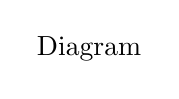
\begin{tikzpicture}
            \node {Diagram};
        \end{tikzpicture}
    \end{center}
        \begin{tasks}(2)
            \task \(\frac{2475}{64}\ \mu\Omega\)
            \task \(\frac{1875}{64}\ \mu\Omega\)
            \task \(\frac{1875}{49}\ \mu\Omega\)
            \task \(\frac{2475}{132}\ \mu\Omega\)
        \end{tasks}


